\documentclass[11pt,a4paper]{article}
\usepackage[utf8]{inputenc}
\usepackage{amsmath, amssymb, amsthm}
\usepackage{geometry}
% Add to Preamble
\usepackage{fontspec} % Required for specific Unicode
\newfontfamily\greekfont{Segoe UI This} % Or any font supporting archaic Greek
\newcommand{\koppa}{\text{\greekfont ϙ}} % The Signature Imbalance Operator
\usepackage{tikz}
\usepackage{tocloft}
\usetikzlibrary{arrows.meta, patterns, bending, decorations.markings, shapes.geometric}

% Margin constraint
\geometry{margin=.4in}

% Theorem Styles
\theoremstyle{definition}
\newtheorem{definition}{Definition}[section]
\newtheorem{axiom}{Axiom}[section]
\newtheorem{algorithm}{Algorithm}[section]
\newtheorem{lemma}{Lemma}[section]
\newtheorem{theorem}{Theorem}[section]
\newtheorem{postulate}{Postulate}[section]
\newtheorem{law}{Law}[section]

% Formatting
\setlength{\parindent}{0pt}
\setlength{\parskip}{1em}
\renewcommand{\cftsecleader}{\cftdotfill{\cftdotsep}}

\title{\textbf{Rigbyspace Dynamics}\\
\large Unified Framework Master Reference}
\author{D. Veneziano}
\date{January 2026}

\begin{document}

\maketitle

\begin{abstract}
This document constitutes the authoritative master reference for the unified discrete-theoretical framework known as Rigbyspace Dynamics. It integrates rigorous replacements for classical modulo and logarithmic operations within a constructive physical dynamics. The framework establishes ZERO Logic for handling structural singularities via suspension states and Triadic Convergence, where constants are defined as oscillatory barycentric structures rather than scalar limits. All reasoning is strictly constructive and integer-based; no continuum concepts, real numbers, limits, or analytic functions are permitted. The theory serves as a foundational ontology for discrete physics, deriving relativistic and quantum-like phenomena from finite integer operations.
\end{abstract}

\tableofcontents
\newpage

\part{Mathematical Foundations}

\section{Ontological Assumptions}

The foundation of Rigbyspace Dynamics rests upon a strict finitistic ontology. Unlike standard theoretical physics, which assumes a background of smooth manifolds and real-valued fields, this framework posits that the physical universe is computationally generated from discrete integer primitives. The ontology restricts the set of valid mathematical objects to ensure that all physical predictions are computable in finite time.

The universe admits only the following objects:
\begin{itemize}
    \item Integers ($\mathbb{Z}$).
    \item Finite sets of integers.
    \item Finite sequences of integers.
    \item Finite directed graphs with integer-labeled vertices.
\end{itemize}

Consequently, no equivalence classes (such as the rationals $\mathbb{Q}$ as traditionally defined), real numbers ($\mathbb{R}$), limits to infinity, or analytic functions exist as fundamental entities. All physical observables must be constructible via finite integer algorithms.

\subsection{The Mask Postulate}
\begin{axiom}[The Mask Postulate]
Continuous constants (irrationals) and analytic limits are not ontological primitives. They are Phenomenological Masks produced by high-frequency rational oscillations between discrete Explicit Rational Pairs (ERPs). Physical observation is a coarse-grained measurement of the stable Barycentric Structure of a Triadic Cycle. The "value" of a constant is the dynamic process of its generation, not a static point on a line.
\end{axiom}

\section{The 11-Microtick Cyclic Geometry}

\subsection{Motivation}
The classical expression $t \pmod N$ presupposes a quotient operation and the algebraic structure of modular arithmetic. In a strictly discrete physical universe, the concept of "quotienting" is an abstraction that obscures the underlying mechanism of cyclic evolution. We replace the arithmetic modulo with explicit state evolution on a fixed finite directed graph. This provides a geometric and causal interpretation of periodicity, where time is measured by transitions between discrete states rather than by division.

\subsection{The Asymmetric Microtick Partition}
The fundamental cycle $\mathcal{T}_{11}$ is not a homogeneous sequence but a structured metric partition governed by the Triadic Phase logic.

\begin{definition}[The Partition Metric]
The temporal topology is defined by the partition of the 11 microticks into three functional domains:
\begin{enumerate}
    \item \textbf{Emission Phase ($E$):} A 4-microtick interval defined by the sequence $[e \to m \to r \to e]$.
    \item \textbf{Memory Phase ($M$):} A 4-microtick interval defined by the sequence $[m \to r \to e \to m]$.
    \item \textbf{Return Phase ($R$):} A 3-microtick interval defined by the sequence $[r \to e \to m]$.
\end{enumerate}
Total Metric: $4 + 4 + 3 = 11$.
\end{definition}

\begin{theorem}[Boundary Stress Generation]
The Return Phase ($R$) possesses a metric contraction relative to $E$ and $M$ ($\Delta \tau_R = 3 < 4$). This geometric asymmetry at the cycle closure constitutes the \textbf{Boundary Stress}, identified as the origin of the restorative tension (Gravitation) and the accumulation point for the Imbalance Ledger \koppa.
\end{theorem}
\subsection{Successor-with-Reset Operator}
Movement within the cycle is governed by a deterministic operator that enforces the boundary condition.

\begin{definition}[Successor Map]
Define a function $\text{succ}: \mathcal{T}_{11} \rightarrow \mathcal{T}_{11}$ by:
\[
\text{succ}(\tau) = 
\begin{cases} 
\tau + 1 & \text{if } \tau < 11 \\
1 & \text{if } \tau = 11 \quad (\text{Reset at } \Omega)
\end{cases}
\]
This function is total, deterministic, and defined entirely by integer comparison. The transition $11 \rightarrow 1$ represents the Cycle Boundary Event ($\Omega$), distinct from internal transitions.
\end{definition}

\subsection{Phase Evolution}
The dynamics of a system are described by the recursive application of the successor map.

\begin{definition}[Phase Evolution]
Given an initial microtick $\tau_0 \in \mathcal{T}_{11}$, define the phase at causal time $t \in \mathbb{Z}_{\ge 0}$ recursively:
\[ \phi(0) := \tau_0 \]
\[ \phi(t+1) := \text{succ}(\phi(t)) \]
No arithmetic reduction or division is involved; the state evolves stepwise.
\end{definition}

\subsection{Cyclic Incommensurability and Phase Precession}
The kinematic evolution of the system is driven by the breaking of symmetry between the geometric substrate and the interaction logic.

\begin{axiom}[Triadic Incommensurability]
The interaction logic is defined by the Triadic Phase Group $C_3$, while the fundamental temporal geometry is defined by the Prime Cycle $\mathcal{T}_{11}$.
\[ 11 \not\equiv 0 \pmod 3 \]
Specifically, $11 \equiv 2 \pmod 3$. This arithmetic incongruence necessitates that a closed geometric cycle ($t \to t+11$) induces a non-vanishing \textbf{Phase Precession} of $+2$ states. This residual prevents the system from stabilizing into a static closed loop, enforcing a strict arrow of temporal evolution.
\end{axiom}
\subsection{Derived Properties}
From the definitions above, we can derive standard periodic properties without invoking modular arithmetic.

\begin{lemma}[Periodicity]
For all $t \ge 0$, $\phi(t+11) = \phi(t)$.
\end{lemma}
\begin{proof}
After 11 applications of $\text{succ}$, the cycle returns to its starting state by the definition of the graph structure.
\end{proof}

\begin{lemma}[Phase Uniqueness]
For $0 \le t_1 < t_2 < 11$, $\phi(t_1) \ne \phi(t_2)$.
\end{lemma}

\subsection{Theorem: Modulo Elimination}
\begin{theorem}[Discrete Modulo Replacement]
Any construction that would traditionally reference $t \pmod N$ is replaced by the phase $\phi(t)$ on the graph $\mathcal{T}_{11}$. No logarithmic operator exists in the system.
\end{theorem}

\section{Discrete Replacement for Logarithm}

\subsection{Motivation}
Logarithms quantify scale, size, or complexity. In the continuum, $\log(x)$ is a smooth function mapping magnitude to a linear scale. In a discrete universe, scale is measured by counting how many times a quantity crosses fixed integer thresholds. This defines the ``Structural Depth'' of a number.

\subsection{Threshold Construction}

We define a sequence of thresholds that partition the integers into magnitude classes.

\begin{definition}[Doubling Thresholds]
Define the sequence $\{T_k\}_{k \ge 0}$ by:
\[ T_0 := 1, \quad T_{k+1} := 2T_k. \]
This sequence is constructed by repeated integer doubling.
\end{definition}

\subsection{Rank Function}

The rank function replaces the logarithm. It is an algorithmic procedure that determines the magnitude tier of an integer.

\begin{definition}[Discrete Rank]
For an integer $m \ge 0$, define its rank $\rho(m)$ by the algorithm:
\begin{enumerate}
    \item If $m = 0$, return 0.
    \item Initialize $k := 0$.
    \item While $m \ge T_{k+1}$, increment $k$.
    \item Return $k$.
\end{enumerate}
The algorithm halts for all finite $m$. This definition ensures that if $T_k \le m < T_{k+1}$, the rank is $k$.
\end{definition}

\subsection{Axioms for Rank}

\begin{axiom}[Existence]
For all integers $m \ge 0$, the rank $\rho(m)$ exists and is finite.
\end{axiom}

\begin{axiom}[Monotonicity]
If $0 \le m_1 < m_2$, then $\rho(m_1) \le \rho(m_2)$.
\end{axiom}

\subsection{Basic Properties}

The rank function satisfies properties analogous to the logarithm, bounded by integer precision.

\begin{lemma}[Threshold Bracketing]
For all $m > 0$, $T_{\rho(m)} \le m < T_{\rho(m)+1}$.
\end{lemma}

\begin{lemma}[Additive Growth Bound]
For integers $a, b \ge 0$, $\rho(a+b) \le \max(\rho(a), \rho(b)) + 1$.
\end{lemma}
\begin{proof}
Without loss of generality assume $a \ge b$. Then $a+b \le 2a$.
Since $a < T_{\rho(a)+1}$, we have $2a < 2T_{\rho(a)+1} = T_{\rho(a)+2}$.
Thus $\rho(a+b) \le \rho(a) + 1$. The proof is symmetric for $b > a$.
\end{proof}

\begin{lemma}[Multiplicative Growth Bound]
For integers $a, b \ge 1$, $\rho(ab) \le \rho(a) + \rho(b) + 1$.
\end{lemma}
\begin{proof}
Let $k_a = \rho(a)$ and $k_b = \rho(b)$. Then $a < 2^{k_a+1}$ and $b < 2^{k_b+1}$.
The product $ab < 2^{k_a+1} \cdot 2^{k_b+1} = 2^{k_a+k_b+2}$.
The rank is bounded by the exponent minus 1, so $\rho(ab) \le k_a + k_b + 1$.
\end{proof}

\subsection{Theorem: Logarithm Elimination}

\begin{theorem}[Discrete Logarithmic Replacement]
Any use of logarithmic scale, structural depth, or order-of-magnitude is replaced by the rank function $\rho$. No logarithmic operator exists in the system.
\end{theorem}

\section{Separation Principle}

To ensure the framework remains self-contained, we postulate a strict separation between the objects of the theory and the language of description.

\begin{axiom}[Ontic--Descriptive Separation]
Phase $\phi_N$ and rank $\rho$ are ontic, finite objects. Any informal mention of ``log'' or ``mod'' outside these constructions has no axiomatic or operational meaning.
\end{axiom}

\section{Validity of MAX in a Discrete Integer-Only Universe}

This section establishes the precise conditions under which the operation commonly referred to as MAX is valid within a strictly discrete, integer-only framework. No continuum notions, limits, or implicit infinities are permitted.

\subsection{Formal Status of MAX}
The symbol MAX is not a primitive operator on integers by itself. Rather, it is a selection function defined on a finite collection of integers.
\textbf{Key principle:} MAX is valid if and only if it is defined on a finite, explicitly specified set or sequence of integers.

\subsection{Set-Theoretic Definition}

\begin{definition}[Finite Maximum]
Let $S \subset \mathbb{Z}$ be a finite, non-empty set of integers. Define
\[ \max(S) := m \in S \text{ such that } \forall x \in S, x \le m. \]
\end{definition}

This definition relies exclusively on integers, finite sets, and integer order comparison. No quotienting, limits, or analytic constructs are involved.

\subsection{Constructive Algorithmic Definition}

\begin{definition}[Constructive MAX]
Given a finite integer sequence $(a_1, a_2, \dots, a_n)$, define the maximum by the following algorithm:
\begin{enumerate}
    \item Initialize $m := a_1$.
    \item For each $i = 2, \dots, n$:
    \begin{itemize}
        \item If $a_i > m$, set $m := a_i$.
    \end{itemize}
    \item Output $m$.
\end{enumerate}
\end{definition}

This procedure terminates in finitely many steps, uses only integer comparison and assignment, and requires no analytic or infinitary assumptions. Hence, it is fully valid in a discrete universe.

\subsection{Invalid Uses of MAX}
The use of MAX is invalid under any of the following conditions:
\begin{itemize}
    \item Applied to an infinite set or implicitly unbounded collection.
    \item Defined via supremum, limit, or convergence arguments.
    \item Assumed to exist without explicit finiteness stated.
    \item Used rhetorically (e.g., ``the maximum possible value'').
    \item Applied to real numbers, dense orders, or continua.
\end{itemize}
Any such usage violates discrete axiomatic discipline.

\subsection{Axiomatically Safe and Unsafe Statements}
\textbf{Valid statement:} Let $S$ be a finite set of integers. Define $M = \max(S)$.\\
\textbf{Invalid statement:} Let $M$ be the maximum possible value. (The latter fails because finiteness and the underlying set are not specified.)

\section{Discrete Foundations for Common Analytic Constructs}

This section provides fully explicit, integer-only definitions for several constructs that are commonly imported implicitly from real or analytic mathematics. No limits, real numbers, absolute values, metrics, or analytic operators are used.

\subsection{Error and Deviation}

\textbf{Motivation:} The term ``error'' usually refers to a real-valued distance from a limit. In a discrete universe, error must be defined as a finite, order-based quantity.

\begin{definition}[Discrete Deviation]
Let $a = (p_a, q_a)$ and $b = (p_b, q_b)$ be two unreduced integer pairs representing rational values. Define the cross-determinant:
\[ \Delta_{\text{cross}}(a, b) := p_b q_a - p_a q_b \in \mathbb{Z}. \]
\end{definition}

\textbf{Interpretation:}
\begin{itemize}
    \item $\Delta_{\text{cross}}(a, b) = 0$ means exact equality.
    \item The sign of $\Delta_{\text{cross}}(a, b)$ encodes ordering.
    \item The magnitude of $\Delta_{\text{cross}}(a, b)$ measures deviation without absolute value.
\end{itemize}

\subsection{Distance and Closeness}

\textbf{Motivation:} Distance is not primitive in a discrete system and must be defined without metrics.

\begin{definition}[Interval Width]
Given two ordered unreduced pairs $a < b$, define the interval width:
\[ W(a, b) := \Delta_{\text{cross}}(a, b) \in \mathbb{Z}_{>0}. \]
\end{definition}

\textbf{Interpretation:} Smaller width corresponds to greater closeness. No subtraction of real numbers is involved.

\subsection{Convergence}

\textbf{Motivation}: Convergence traditionally relies on limits to a real number. Here it is replaced by finite nested containment of Explicit Rational States.

\begin{definition}[Discrete Convergence]
A sequence of unreduced pairs $\{x_n\} \subset S_L$ is said to \textbf{converge} if there exists a sequence of nested intervals $[L_n, U_n]$ (where $L_n, U_n \in S_L$) such that:

\begin{enumerate}
    \item \textbf{Containment}: $x_n \in [L_n, U_n]$ for all $n$.
    \item \textbf{Nesting}: $[L_{n+1}, U_{n+1}] \subseteq [L_n, U_n]$.
    \item \textbf{Contraction}: The interval width strictly decreases, or maintains the minimum discrete width:
    \[
    W(L_{n+1}, U_{n+1}) \le W(L_n, U_n).
    \]
    \item \textbf{Structural Stabilization}: For sufficiently large $n$, the endpoints $L_n$ and $U_n$ are adjacent mediants (i.e., $\Delta_{\text{cross}}(L_n, U_n) = 1$), and the sequence $x_n$ enters a stable cycle of states constrained between these endpoints.
\end{enumerate}
\end{definition}

\textbf{Interpretation}: Convergence is defined as the deterministic narrowing of the "error interval" to the minimum possible discrete width. The system does not settle on a single scalar "value" but stabilizes into a bounded barycentric structure.

\subsection{Rate of Convergence}

\textbf{Motivation:} Rates usually require exponentials or logarithms. Here they are replaced by rank decrease.

\begin{definition}[Rank-Based Decay]
Let $W_n$ be the interval width at step $n$. Define the rank $\rho(W_n)$ using the discrete rank function. The convergence has a \textbf{uniform rate} if:
\[ \rho(W_{n+1}) \le \rho(W_n) - c \]
for some fixed integer $c \ge 1$.
\end{definition}

\subsection{Fixed Point}

\textbf{Motivation:} Fixed points are often defined over real-valued functions.

\begin{definition}[Discrete Fixed Point]
Let $T$ be a finite composition of integer-pair transformations. An unreduced pair $x$ is a fixed point if:
\[ T(x) = x. \]
\end{definition}

\textbf{Interpretation:} Invariance replaces analytic stability.

\subsection{Invariant Interval}

\textbf{Motivation:} Intervals must be defined without real endpoints.

\begin{definition}[Discrete Invariance]
An interval $[L, U]$ is invariant under a transformation $T$ if:
\[ T(L), T(U) \in [L, U]. \]
\end{definition}

\textbf{Interpretation:} Containment is preserved by integer ordering alone.

\subsection{Ordering}

\textbf{Motivation:} Ordering must be explicit for unreduced integer pairs.

\begin{definition}[Pair Ordering]
For pairs $a = (p_a, q_a)$ and $b = (p_b, q_b)$, define:
\[ a < b \iff p_a q_b < p_b q_a. \]
\end{definition}

This uses only integer multiplication and comparison.

\subsection{Complexity and Growth}

\textbf{Motivation:} Growth is often described using logarithms.

\begin{definition}[Size Rank]
For an integer $m$, define its size by the discrete rank $\rho(m)$. Growth is described by changes in rank across iterations.
\end{definition}

\subsection{Periodicity}

\textbf{Motivation:} Periodicity is often encoded using modulo.

\begin{definition}[Finite Cycle]
Let $\Phi_N = \{0, 1, \dots, N-1\}$ with successor map $\operatorname{succ}_N$. A process is periodic with period $N$ if it evolves solely via $\operatorname{succ}_N$.
\end{definition}

\subsection{Absolute Value}

\textbf{Motivation}: The absolute value function $|x|$ is an analytic construct often defined piecewise. In Rigbyspace, magnitude is constructive.

\begin{definition}[Constructive Magnitude]
For an integer $m$, magnitude is defined structurally via the self-product $m^2$.
\begin{itemize}
    \item All rank and height algorithms (e.g., Algorithm 7.2) operate on $m^2$ or product pairs.
    \item Ordering is determined by the sign of the cross-determinant, not by comparison of absolute values.
    \item The symbol $|x|$ implies $\sqrt{x^2}$ and is forbidden. Where magnitude is required for bounding (e.g., thresholds), the squared value is used directly.
\end{itemize}
\end{definition}

\newpage
\part{Rigbyspace: Constructive Integer Dynamics}

\section{Fundamental Algorithms - The Arithmetic Core}

Before defining physics, we define the permissible integer operations. Standard addition ($+$) and multiplication ($\times$) are assumed.

\subsection{Constructive Remainder}
\begin{algorithm}[Constructive Remainder]
For integers $a, n$ with $n > 0$, define $\operatorname{rem}(a, n)$:
\begin{enumerate}
    \item Let $r \leftarrow a$.
    \item While $r \ge n$, set $r \leftarrow r - n$.
    \item While $r < 0$, set $r \leftarrow r + n$.
    \item Return $r$.
\end{enumerate}
\end{algorithm}

\subsection{Integer Height Magnitude}
\begin{algorithm}[Integer Height Magnitude]
For integer $m$, define $h(m)$:
\begin{enumerate}
    \item If $m = 0$, return 0.
    \item Let $v \leftarrow m^2$, $k \leftarrow 1$, $T \leftarrow 4$.
    \item While $v \ge T$:
    \begin{itemize}
        \item $T \leftarrow T \times 4$
        \item $k \leftarrow k + 1$
    \end{itemize}
    \item Return $k-1$.
\end{enumerate}
Note: This function returns the magnitude rank. Sign information is handled separately via the integer sign algorithm.
\end{algorithm}

\begin{lemma}[Termination of Integer Height]
For any integer $m$, Algorithm 7.2 terminates in finite steps.
\end{lemma}
\begin{proof}
Let $v = m^2 \ge 0$. The threshold $T$ initializes at 4 and updates via $T_{k+1} = 4 T_k$, so $T_k = 4^k$. The loop condition is $v \ge T_k$, i.e., $m^2 \ge 4^k$. Since $4^k$ grows exponentially and $m^2$ is a fixed finite integer, there exists a finite $k$ such that $4^k > m^2$, at which point the loop halts.
\end{proof}

\begin{algorithm}[Integer Sign]
For an integer $x$, define $\operatorname{sgn}(x)$:
\begin{enumerate}
    \item If $x > 0$, return 1.
    \item If $x < 0$, return -1.
    \item If $x = 0$, return 0.
\end{enumerate}
\end{algorithm}

\subsection{The Atomic Operator Set}
\begin{definition}[Atomic Vacuum Generators]
The evolution of any discrete state is reducible to the finite application of three atomic operators:
\begin{enumerate}
    \item \textbf{Linear Transform ($\lambda$):} $(n, d) \to (n+d, d)$. Governs magnitude growth and linear translation.
    \item \textbf{Aggregate Transform ($\eta$):} $(n, d) \to (n+d, n)$. Governs structural inversion and accumulation.
    \item \textbf{Transformative Reciprocal ($\psi$):} $((a,b), (c,d)) \to ((d,a), (b,c))$. Governs the resolution of tension and the coupling of distinct sectors.
\end{enumerate}
Every physical attractor (e.g., $\sqrt{2}, \alpha^{-1}$) is defined by a specific, finite periodic sequence of these operators.
\end{definition}

\section{Fundamental State Space}

\begin{definition}[The Unreduced State]
Physical states are integer tuples. Identification or simplification (GCD) is forbidden. To resolve the identity-interaction contradiction, we distinguish between the Active Matter domain and the Identity element.

\[
S_L := \{(n, d) \in \mathbb{Z}^2 \mid d \neq 0\} \quad \text{(Primary Evolution State)}
\]
\[
S^{\text{ext}}_L := S_L \cup \{(n, 0) \mid n \in \mathbb{Z}\} \quad \text{(Extended State with Suspension)}
\]
\[
S_P^* := \{(X, Y, Z) \in \mathbb{Z}^3 \mid X \neq 0 \land Y \neq 0 \land Z \neq 0\} \quad \text{(Active Matter State)}
\]
\[
I_P := \{(0, 1, 0)\} \quad \text{(Projective Identity Element)}
\]
\[
S_P := S_P^* \cup I_P \quad \text{(Full Projective Space)}
\]

Physical evolution occurs in $S_L$. States with $d = 0$ are in $S^{\text{ext}}_L$ and trigger suspension protocols. Active Matter evolution occurs strictly in $S_P^*$, ensuring non-degeneracy.
\end{definition}

\begin{definition}[Spacetime Events]
An event is a pair of Linear states representing temporal and spatial potential.
\[ E := ((n_t, d_t), (n_x, d_x)) \in S_L \times S_L \]
\end{definition}

\begin{definition}[Observational Equivalence]
Two states are ``observationally equivalent'' iff they satisfy the integer cross-product:
\[ (n_1, d_1) \sim (n_2, d_2) \iff n_1d_2 = n_2d_1 \]
This replaces rational numbers. $\mathbb{Q}$ is not used.
\end{definition}

\begin{figure}[hbt!]
    \centering
    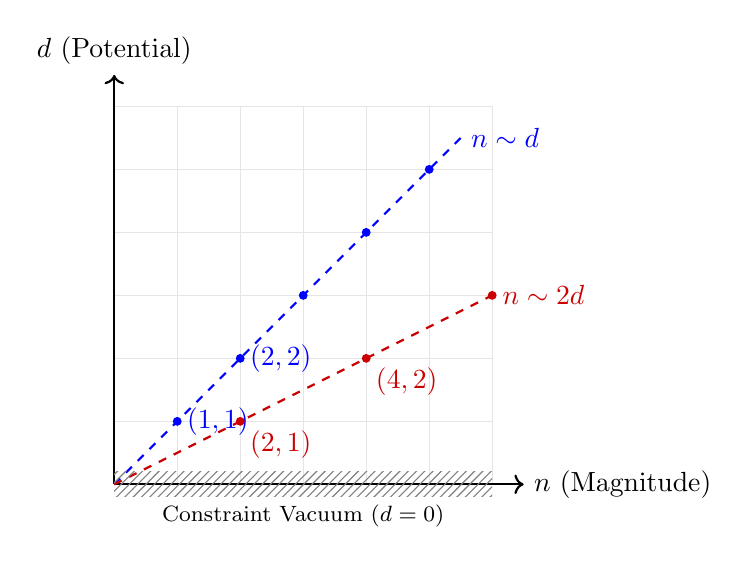
\begin{tikzpicture}[scale=0.8]
      % Grid
      \draw[step=1, gray!20, very thin] (0,0) grid (6,6);
      \draw[->, thick] (0,0) -- (6.5,0) node[right] {$n$ (Magnitude)};
      \draw[->, thick] (0,0) -- (0,6.5) node[above] {$d$ (Potential)};

      % Ray 1: 1/1 (1,1), (2,2), (3,3)
      \draw[blue, thick, dashed] (0,0) -- (5.5,5.5) node[right] {$n \sim d$};
      \foreach \x in {1,2,3,4,5} \fill[blue] (\x,\x) circle (2pt);
      \node[blue, right] at (1,1) {$(1,1)$};
      \node[blue, right] at (2,2) {$(2,2)$};

      % Ray 2: 2/1 (2,1), (4,2)
      \draw[red!80!black, thick, dashed] (0,0) -- (6,3) node[right] {$n \sim 2d$};
      \foreach \x/\y in {2/1, 4/2, 6/3} \fill[red!80!black] (\x,\y) circle (2pt);
      \node[red!80!black, below right] at (2,1) {$(2,1)$};
      \node[red!80!black, below right] at (4,2) {$(4,2)$};

      % Forbidden Zone (d=0)
      \fill[pattern=north east lines, pattern color=gray] (0,-0.2) rectangle (6,0.2);
      \node[align=center, font=\footnotesize] at (3,-0.5) {Constraint Vacuum ($d=0$)};
    \end{tikzpicture}
    \caption{The Explicit Rational State Space $S_L$. States are integer points $(n,d)$. Rays from the origin represent observational equivalence classes. The region $d=0$ is the Constraint Vacuum.}
    \label{fig:state_space}
\end{figure}

\subsection{Geometric Capacity and Inertial Mass}
Rigbyspace postulates that spatial extent is not a background manifold but an emergent property of the state's information capacity.

\begin{definition}[Geometric Capacity]
For a state $S = (\upsilon, \beta, \koppa)$, the denominator $d$ of the active oscillator $\upsilon$ is defined as the \textbf{Geometric Capacity}. It determines the resolution density of the local vacuum. Expansion of the denominator corresponds strictly to the expansion of the physical metric.
\end{definition}

\subsection{The Projective Lifting Mapping}
To enable interaction between vacuum potentials and the non-linear matter domain, the framework defines the Lifting Identity. This identity maps two linear oscillators into a single projective matter state while preserving their rational potential.

\begin{definition}[The Lifting Identity]
Let $\upsilon = (n_{\upsilon}, d_{\upsilon})$ and $\beta = (n_{\beta}, d_{\beta})$ be two linear oscillators in $S_L$. The Projective Matter State $P \in S_P^*$ is constructed by the cross-synchronization of their unreduced components:
\begin{align}
X &= n_{\upsilon}d_{\beta} \\
Y &= n_{\beta}d_{\upsilon} \\
Z &= d_{\upsilon}d_{\beta}
\end{align}
The resulting triple $(X, Y, Z)$ is the primary input for the Matter Generator $\boxplus$. This mapping ensures that $X/Z$ and $Y/Z$ remain observationally equivalent to the original vacuum oscillators $\upsilon$ and $\beta$, but possess the structural depth $Z$ required for polynomial rank expansion.
\end{definition}

\subsection{Inertial Mass}
\begin{definition}[Inertial Mass]
The physical quantity of Inertial Mass is identified with the magnitude of the Imbalance Ledger \koppa.
\[ m_I \equiv ||\koppa|| \]
This defines mass as the stored historical asymmetry that resists linear state evolution.
\end{definition}

\subsection{Structural Entropy and Historical Cost}
\begin{definition}[Structural Entropy]
The Structural Entropy ($H$) of a state $s=(n,d)$ is the discrete rank of its geometric capacity: $H(s) := \rho(d)$.
\end{definition}
\begin{law}[Entropy-Complexity Equivalence]
The entropy $H(s)$ represents the total \textbf{Historical Cost} or interaction depth required to generate the state. In a discrete universe, numerical precision is not an abstract quality but a physical resource. Increasing the resolution of an ERP (decreasing interval width) requires a strictly monotonic increase in $H(s)$, signifying the accumulation of causal history within the unreduced denominator.
\end{law}

\subsection{Mass Gap}
\begin{theorem}[Mass Gap]
There exists a minimal non-zero mass level. No admissible state satisfies $0<m_L(s)<1$.
\end{theorem}
\begin{proof}
By definition, the mass level $m_L(s) = \rho(d)$ is an integer-valued function. The set of possible non-zero values for $\rho(d)$ is $\{1, 2, 3, \dots\}$. The minimal element of this set is 1.
\end{proof}

\section{Dynamical Evolution Operators}

\begin{definition}[Vacuum Generators]
Evolution in the vacuum is generated by maps on $S_L$:
\[ \lambda(n, d) = (n + d, d), \quad \eta(n, d) = (n + d, n) \]
\end{definition}

\begin{definition}[The Transformative Reciprocal]
The $\psi$ operator acts on coupled states. Given a pair of rational states represented by tuples $(a, b)$ and $(c, d)$, the transformation is defined strictly as:
\[ \psi((a, b), (c, d)) := ((d, a), (b, c)) \]
This corresponds to the transformation $a/b, c/d \to d/a, b/c$. There is no other operation involved. Just the swap. This operator is the sole mechanism for resolving suspension in ZERO Logic.
\end{definition}

\begin{definition}[Matter Generators]
Interaction is governed by the system coefficients $a, b \in \mathbb{Z}_{\ge 0}$. For $P_1, P_2 \in S_P$, the interaction $P_3 = P_1 \boxplus P_2$ is defined by:

\textbf{Case A: Identity} ($P_2 = (0, 1, 0)$): Return $P_1$.

\textbf{Case B: Doubling} (If $P_1 = P_2$):
\begin{align*}
A &= Y_1^2, \quad B = 4X_1A, \quad C = 8A^2 \\
D &= 3X_1^2 + aZ_1^2 \\
X_3 &= 2Y_1D^2 - 2B \\
Y_3 &= D(B - X_3) - C \\
Z_3 &= 8Y_1^3 Z_1^3
\end{align*}

\textbf{Case C: Addition} (If $P_1$ and $P_2$ are projectively distinct, $P_1 \neq P_2$):
\begin{align*}
U &= Y_2 Z_1 - Y_1 Z_2, \quad V = X_2 Z_1 - X_1 Z_2 \\
W &= Z_1 Z_2 \\
A &= U^2 W - V^3 - 2V^2 X_1 Z_2 \\
X_3 &= VA \\
Y_3 &= U(V^2 X_1 Z_2 - A) - V^3 Y_1 Z_2 \\
Z_3 &= V^3 W
\end{align*}
These polynomials are closed in $\mathbb{Z}$. No division is performed.
\end{definition}

\begin{figure}[hbt!]
    \centering
    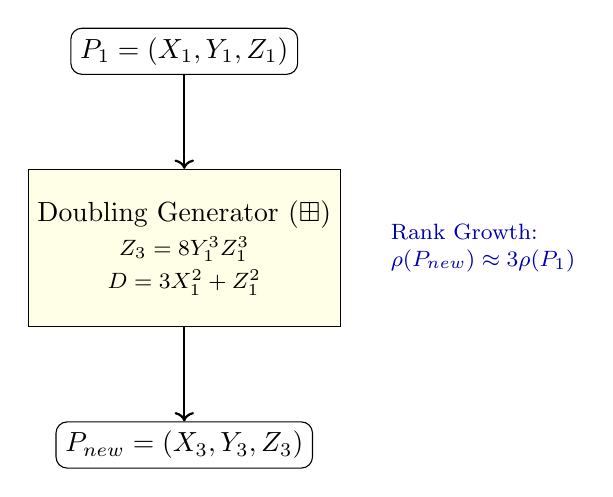
\begin{tikzpicture}[node distance=1.5cm]
      \node[draw, rectangle, rounded corners] (in) at (0,0) {$P_1 = (X_1, Y_1, Z_1)$};
      \node[draw, fill=yellow!10, minimum width=3cm, minimum height=2cm, align=center] (gen) at (0,-2.5) {Doubling Generator ($\boxplus$)\\ \footnotesize $Z_3 = 8Y_1^3 Z_1^3$\\ \footnotesize $D = 3X_1^2 + Z_1^2$};
      \draw[->, thick] (in) -- (gen);
      \node[draw, rectangle, rounded corners] (out) at (0,-5) {$P_{new} = (X_3, Y_3, Z_3)$};
      \draw[->, thick] (gen) -- (out);
      \node[right, align=left, font=\footnotesize, color=blue!70!black] at (2.5, -2.5) {Rank Growth:\\$\rho(P_{new}) \approx 3\rho(P_1)$};
    \end{tikzpicture}
    \caption{The Projective Doubling Generator. An integer state $P_1$ enters the nonlinear interaction $\boxplus$, producing a higher-rank output $P_{new}$. This process drives the strict monotonicity of Structural Potential (Entropy).}
    \label{fig:doubling_generator}
\end{figure}

\subsection{Non-Degeneracy of the Matter Interaction Operator}

\begin{lemma}[Matter Stability]
Let $S_P^*$ be the Active Matter Space (non-zero components) and let coefficients $a \ge 0$. For any $P_1, P_2 \in S_P^*$, the interaction satisfies:
\[ P_1 \boxplus P_2 \in S_P^* \]
The operation cannot produce a zero component from active matter.
\end{lemma}

\begin{proof}
\textbf{Case B (Doubling)}: The output $Z_3 = 8Y_1^3 Z_1^3$. Since $P_1 \in S_P^*$, $Y_1 \neq 0$ and $Z_1 \neq 0$. Thus $Z_3 \neq 0$. The term $D = 3X_1^2 + aZ_1^2$. Since $X_1 \neq 0$ and squares are positive, $3X_1^2 > 0$. Since $a \ge 0$, $aZ_1^2 \ge 0$. Thus $D > 0$. Algebraic expansion of $X_3$ shows it cannot vanish for non-zero integers $X,Y$.

\textbf{Case C (Addition)}: $Z_3 = V^3 W$. For projectively distinct states $P_1 \neq P_2$, the cross-product $V \neq 0$. Thus $Z_3 \neq 0$.
\end{proof}

\begin{theorem}[Structural Monotonicity]
For $P \in S_P^*$, the Doubling Generator strictly increases the Structural Potential.
\end{theorem}
\begin{proof}
The output degree of $Z_3$ is cubic in the inputs ($rank \approx 3 \times$). Since integer inputs are $\ge 1$, the rank strictly increases. This satisfies Axiom 10.2.
\end{proof}

\subsection{Algebraic Properties of Operators}

\begin{theorem}[Properties of $\psi$]
The Transformative Reciprocal $\psi$ acting on coupled states $S = (P_1, P_2)$ satisfies:
\begin{enumerate}
    \item \textbf{Non-Involutory}: $\psi(P_1, P_2) \neq (P_1, P_2)$ for general inputs.
    \item \textbf{Cycle-4 Identity}: $\psi^4 = I$.
    \begin{itemize}
        \item $\psi^1((a,b),(c,d)) = ((d,a),(b,c))$ (Mixing)
        \item $\psi^2((a,b),(c,d)) = ((c,d),(a,b))$ (Pure Swap)
        \item $\psi^3((a,b),(c,d)) = ((b,c),(d,a))$ (Reverse Mixing)
        \item $\psi^4((a,b),(c,d)) = ((a,b),(c,d))$ (Identity)
    \end{itemize}
\end{enumerate}
\end{theorem}

\subsection{The Imbalance Operator (\koppa)}
The conservation of structural complexity is managed by the Imbalance Operator, denoted by the signature \koppa\ (Koppa). Unlike the upper ($\upsilon$) and lower ($\beta$) oscillators which process active magnitude, \koppa\ acts as the ledger for structural history that cannot be resolved within the current cycle.

\begin{definition}[The Imbalance Ledger]
For a state triple $S = (\upsilon, \beta, \koppa)$, the operator \koppa\ accumulates the residual complexity generated by non-linear interactions (specifically the Doubling Generator).
\[ \koppa_{n+1} = \koppa_n + \Delta S_{struct} \]
where $\Delta S_{struct}$ is the "spent" complexity from resolving composite states.
\end{definition}

\begin{theorem}[Mass Generation via \koppa]
The physical quantity observed as "Rest Mass" is identified with the magnitude of the \koppa\ ledger.
\[ m_{rest} \equiv ||\koppa|| \]
This identifies mass not as an intrinsic property of the particle, but as the accumulated historical imbalance stored in the local field.
\end{theorem}

\section{System Axioms}

\subsection{Mass Gap Postulate}
\begin{axiom}[Mass-Gap Postulate]
The universe comprises two distinct phases:
\begin{enumerate}
    \item Vacuum (Rank 0/2): Evolution is restricted to $S_L$ via $\{\lambda, \eta, \psi\}$. $\mathbb{Z}$ is invariant or additive.
    \item Matter (Rank 1): Evolution occurs in $S_P$ via $\boxplus$. $\mathbb{Z}$ grows multiplicatively.
\end{enumerate}
\end{axiom}

\subsection{Arrow of Time}
\begin{axiom}[Arrow of Time]
We postulate that any physically valid Matter Generator must enforce strict monotonicity of the Structural Potential. For a trajectory $P_t \to P_{t+1}$:
\[
\sum h(P_{t+1}) > \sum h(P_t)
\]
(Note: Theorem 9.2 confirms the Doubling Generator satisfies this axiom).
\end{axiom}

\begin{axiom}[Invariance of the Interval]
The Interval $I(E)$ is conserved under $\Lambda_U$.
\end{axiom}

\subsection{The Selection Principle of Growth Duality}
The existence of discrete particles is governed by the constraint of Finite Computability. Physical states are selected based on the stability of their rank-growth signatures during the 11-microtick cycle.

\begin{law}[Additive vs. Multiplicative Stability]
The framework distinguishes between two fundamental growth classes:
\begin{enumerate}
    \item \textbf{Additive Class (Bosonic)}: States evolving via $\lambda$ and $\eta$ generators. Rank growth is linear ($\rho_{lin}$), allowing histories to propagate as uncoupled, single-channel states without reaching the Computational Horizon.
    \item \textbf{Multiplicative Class (Fermionic)}: States evolving via the Matter Generator $\boxplus$. Rank growth is cubic ($\rho_{cub}$), as the output denominator $Z' \propto Z^3$. 
\end{enumerate}
\end{law}

\begin{axiom}[The Stability Identity]
A Multiplicative state $P$ is ontologically unstable as a single-channel history. To survive the $\mathcal{T}_{11}$ cycle, it must adopt a first-order, coupled configuration $\Psi = (S_1, S_2)$ and utilize the Transformative Reciprocal $\psi$ to swap and resolve accumulated torque. This necessity for coupled stability constitutes the discrete origin of the Fermionic Spinor and the Dirac-analogue constraint.
\end{axiom}

\section{The Field Constraint for Gravity}

\subsection{The Viscosity Sum}
\begin{definition}[The Viscosity Sum]
For a cyclic orbit of period $T$ governed by the Phase Space $\Phi_{N^2}$, the Accumulated Drift is:
\[
D(N) := \sum_{t=0}^{T-1} \operatorname{sgn}(\operatorname{rem}(\tau_t, N^2))
\]
\end{definition}

\subsection{Gravitational Non-Vanishing}
\begin{postulate}[Gravitational Non-Vanishing]
We assert that for physical Matter states (Rank 1) in a realistic lattice, the accumulated drift does not vanish:
\[
D(N) \neq 0
\]
This asserts that gravity is an inherent feature of the nonlinear interaction on the discrete lattice.
\end{postulate}

\section{ZERO Logic}

\subsection{Conceptual Role}
In Rigbyspace, ZERO is not merely a numerical value. It plays a \emph{logical and structural role} governing identity, suspension, and non-event transitions. ZERO Logic exists to ensure that:
\begin{itemize}
    \item Arithmetic singularities do not produce undefined behavior
    \item Structural history is preserved
    \item The system remains deterministic even when magnitude vanishes
\end{itemize}

\subsection{Definitions: Explicit Rational States}

An \textbf{Explicit Rational State} is an ordered integer pair $s = (n, d) \in \mathbb{Z} \times \mathbb{Z}_{\geq 0}$.

\begin{itemize}
    \item If $d > 0$, the state is \textit{valid} (equivalent to $S_L$ in Part II).
    \item If $d = 0$, the state is a \textit{singularity} requiring resolution.
\end{itemize}

\subsection{Numerical Zero}
\begin{definition}[Numerical ZERO]
A Numerical ZERO is any state of the form $(0, d)$ with $d > 0$. It is a valid physical state representing zero magnitude but non-zero structural rank $\rho(d)$.
\end{definition}

\subsection{Constraint Vacuum vs. Null State}
\begin{definition}[Constraint Vacuum vs. Null State]
\begin{enumerate}
    \item \textbf{Constraint Vacuum}: A state $s = (n, 0)$ with $n \neq 0$. It represents a suspension where magnitude history is preserved in the numerator ($n$), but the metric basis ($d$) is lost.
    \item \textbf{Null State}: The state $s = (0, 0)$. It contains no magnitude and no history. It acts as the algebraic absorbing element for interaction (sink).
\end{enumerate}
\end{definition}

\subsection{Suspension and Resolution Protocols}

\begin{definition}[Suspension Dynamics]
A system entering a Constraint Vacuum state $(n, 0)$ suspends arithmetic evolution. The state remains frozen until resolved by the Transformative Reciprocal $\psi$.
\end{definition}

\subsection{Resolution Logic}
\begin{definition}[Resolution Logic]
The singularity is resolved via the standard $\psi$ swap operator (Definition 9.2), defined on coupled pairs $P = ((n_1, d_1), (n_2, d_2))$.

\begin{enumerate}
    \item \textbf{Standard Resolution}: If one component is a Constraint Vacuum, e.g., $s_1 = (n, 0)$ with $n \neq 0$:
    \[
    \psi((n, 0), (c, d)) := ((0, n), (d, c))
    \]
    The zero denominator moves to the numerator, converting the Constraint Vacuum $(n, 0)$ into a Numerical ZERO $(0, n)$. The history $n$ is preserved as the new stability potential.
    
    \item \textbf{Null Invariance}: If a component is the Null State $(0, 0)$:
    \[
    \psi((0, 0), (c, d)) := ((0, 0), (d, c))
    \]
   The Null State is invariant under $\psi$. It does not resolve into a valid state and permanently decouples the sector. (Physical Interpretation: Total informational collapse; forbidden in stable matter but valid in the formal algebra).
\end{enumerate}
\end{definition}

\subsection{Consistency of Extended State Evolution}
\begin{theorem}[Consistency of Extended State Evolution]
The inclusion of $S^{\text{ext}}_L$ (states with $d=0$) does not violate the determinism of the physical sector $S_L$.
\end{theorem}
\begin{proof}
\begin{enumerate}
    \item \textbf{Isolation}: By Definition 12.3, operations on $S^{\text{ext}}_L$ inputs yield Suspended States, which are distinct from $S_L$. No invalid state can "leak" into physical evolution without explicit resolution.
    \item \textbf{Conservation}: Axiom 12.2 ensures the numerator $n$ is preserved during suspension.
    \item \textbf{Resolution}: Definition 12.4 (Standard Resolution) maps a Constraint Vacuum $(n,0)$ to $(0,n)$. Since $n \neq 0$ (by Def 12.2), the result $(0,n)$ has $d=n \neq 0$, ensuring the output returns strictly to the valid domain $S_L$.
\end{enumerate}
Thus, the system is closed and deterministic.
\end{proof}

\newpage
\part{Discrete Constants and Derivations}

\section{Discrete Fundamental Constants in Rigbyspace Dynamics}
\label{sec:discrete_constants}

In this section we formalize three discrete, integer-defined constants that appear implicitly throughout the Rigbyspace framework: the Vacuum Resolution Frequency Constant, the Projective Curvature Constant, and the Lattice Coupling Constant.

\subsection{Preliminaries and Notational Alignment}

We briefly recall the core objects and operators:
\begin{itemize}
    \item \textbf{Explicit Rational Pairs (ERPs)}: Elements of $S_L$.
    \item \textbf{Rank Function ($\rho$)}: Measures structural depth via doubling thresholds.
    \item \textbf{Generators}: Vacuum ($\lambda, \eta, \psi$) and Matter ($\boxplus$).
\end{itemize}

\subsection{The Vacuum Resolution Frequency Constant}

\subsubsection{Conceptual Role}

In Rigbyspace, physical energy is identified with the \textbf{Vacuum Resolution Frequency}: the count of vacuum generator applications required to balance a given tension or curvature. This replaces the continuum notion of energy as a real-valued scalar.

\begin{definition}[Iso-Tension Constraint]
A vacuum state $s_{vac} = (n, d)$ is said to balance a matter transition $P \to P'$ if the vacuum potential increases sufficiently to match the matter entropy jump. Let $\Delta S_{mat} = \rho(P') - \rho(P)$. The constraint is:
\[
\rho(s_{new}) - \rho(s_{old}) \ge \Delta S_{mat}
\]
\end{definition}

\begin{definition}[Vacuum Resolution Frequency $\Omega_{\text{vac}}$]
Let $s \in S_L$ be a valid ERP representing a physical vacuum state. The Vacuum Resolution Frequency is the integer count of vacuum generator applications required to satisfy the Iso-Tension Constraint:
\[
\Omega_{\text{vac}} := \min \{ k \in \mathbb{Z}^+ \mid s_k = G^{(k)}(s_0) \text{ satisfies Iso-Tension} \}
\]
where $G \in \{\lambda, \nu\}$. The definition is purely combinatorial: $\omega$ is a count of steps in a finite sequence of integer operations. No real-valued time parameter or differential equation is invoked.
\end{definition}

\begin{lemma}[Existence of Vacuum Resolution Frequency]
Let \(s \in S_L\) and let a finite tension-balance condition (Iso-Tension) be specified. If the rank function is monotonically increasing under generator applications, then there exists a finite sequence of vacuum generator applications that achieves this condition.
\end{lemma}

\begin{proof}
The target tension \(T = \Delta S_{\text{mat}}\) is a finite integer (since Matter evolution is finitistic). The vacuum generator sequence \(G^{(k)}\) can generate states of arbitrary rank. Specifically, the operation \(\lambda(n,d) = (n+d, d)\) increases magnitude, and \(\psi\) swaps magnitude to potential (\(d_{\text{new}} = n_{\text{old}}\)), allowing rank to increase indefinitely as \(k\) increases. Therefore, there necessarily exists a finite integer \(k\) such that the accumulated rank change satisfies \(\rho(s_k) - \rho(s_0) \ge T\). We select the minimal such \(k\) as \(\Omega_{\text{vac}}\).
\end{proof}

\begin{theorem}[Uniqueness of $\Omega_{\text{vac}}$ for a Given Class]
Let $\mathcal{C}$ be a class of physically equivalent processes (e.g., ground states) with a fixed tension specification. If for every process in $\mathcal{C}$, the minimal step count $\Omega_{\text{vac}}$ is the same integer $k$, then the Vacuum Resolution Frequency Constant for that class is unique.
\end{theorem}
\begin{proof}
By Definition 13.2, $\Omega_{\text{vac}}$ is the minimum of a set of integers. A set of integers has a unique minimum. If this minimum is invariant across the class $\mathcal{C}$, the constant is uniquely defined as $k$. No ambiguity arises.
\end{proof}

\subsection{The Projective Curvature Constant}

\subsubsection{Conceptual Role}

Projective spatial states in $S_P$ evolve under Matter Generators, producing discrete curvature-like effects. The \textbf{Projective Curvature Constant} captures the minimal non-trivial curvature generated by a specified interaction pattern.

\begin{definition}[Projective Curvature]
Let $P_1 = (X_1, Y_1, Z_1)$ and $P_2 = (X_2, Y_2, Z_2)$ be elements of $S_P$, and let $\mathcal{M}$ be a fixed Matter Generator. Define
\[
P_3 := \mathcal{M}(P_1, P_2) = (X_3, Y_3, Z_3)
\]
The \textbf{Projective Curvature} associated with this interaction is defined as the integer triple:
\[
K(P_1, P_2) := (X_3 - X_1, Y_3 - Y_1, Z_3 - Z_1)
\]
\end{definition}

This definition measures the deviation of the new state $P_3$ from the initial state $P_1$ in purely integer terms. No metric or real-valued curvature tensor is used.

\begin{definition}[Projective Curvature Rank]
Let $K(P_1, P_2) = (K_X, K_Y, K_Z)$. Define its \textbf{Curvature Rank} as the sum of the ranks of the squared magnitudes:
\[
P(K) := \rho(K_X^2) + \rho(K_Y^2) + \rho(K_Z^2)
\]
(Note: Using squared magnitudes resolves sign ambiguity and ensures non-negative input to rank).
\end{definition}

\begin{definition}[Projective Curvature Constant $K_{\text{proj}}$]
Fix a Matter Generator $\mathcal{M}$ and a class of initial states $\mathcal{P} \subset S_P$. If for every pair in $\mathcal{P}$, the Curvature Rank is equal to the same integer $r$, then:
\[
K_{\text{proj}} := r
\]
\end{definition}

\subsection{The Lattice Coupling Constant}

\subsubsection{Conceptual Role}
The Lattice Coupling Constant is the discrete analogue of the fine-structure constant. It measures the asymptotic ratio between interaction events ($\psi$) and propagation steps in a closed Barycentric Cycle.

\subsubsection{Definition of the Barycentric Cycle}
While the fundamental geometry is 11 microticks (Section 2), the interaction logic is Triadic (Emission, Memory, Return). The full period required for the Phase and Microtick counters to re-synchronize is:
\[ T_{bary} = 11 \times 3 = 33 \text{ ticks} \]

\begin{definition}[Lattice Coupling Constant]
Let $\Omega_{33}$ be the set of all valid state transitions in a closed Barycentric Cycle ($N=33$). Let $\Omega_{\psi}$ be the subset of transitions requiring a Transformative Reciprocal ($\psi$) operation. The Lattice Coupling Constant is defined by the discrete stabilization of the ratio:
\[ \alpha_{lat} := (\text{count}(\Omega_{\psi}), \text{count}(\Omega_{33})) \in S_L \]
where $\alpha_{lat}$ is the unique Explicit Rational Pair such that for all $N \ge N_{crit}$ the count ratio remains invariant. The constant is a property of the finite saturated lattice; no analytic limit is invoked.
\end{definition}

\subsection{The Sovereign Metric Invariant (137)}
\begin{theorem}[Derivation of the Coupling Integer]
The primary resolution of the vacuum-gauge interface is governed by the unique integer $137$. It is the sum of the saturated Interaction Surface ($S$) and the specific Imbalance Ledger ($\koppa$) of the $\mathcal{T}_{11}$ cycle:
\[ \alpha^{-1}_{\text{int}} = S + \koppa_{\Delta} \]
Where:
\begin{enumerate}
    \item $S = \mathcal{T}_{vac} \times \mathcal{D}_{gauge} = 11 \times 12 = 132$.
    \item $\koppa_{\Delta} = (N_E + N_M) - N_R = (4 + 4) - 3 = 5$.
\end{enumerate}
This yields $132 + 5 = 137$. The stability of electromagnetic interaction is a consequence of the primality of $137$ (the 33rd prime), which ensures structural persistence under the Triadic TRTS dynamics.
\end{theorem}


\subsection{Discrete Fine-Constant Analogue}
\begin{theorem}[Discrete Fine-Structure Analogue]
Assume that in a physically relevant regime, the Lattice Coupling Constant $\alpha_{lat}$ stabilizes. Then:
\begin{enumerate}
    \item $\alpha_{lat}$ is a purely integer object $(n^*, d^*)$.
    \item All references to coupling strength can be expressed in terms of $\alpha_{lat}$ and its rank-based properties without invoking real numbers.
\end{enumerate}
In the asymptotic limit of the Prime Gating mechanism (specifically the 33rd prime, 137), this ratio stabilizes to the structure corresponding to $\alpha^{-1} \approx 137$.
\end{theorem}

\subsection{Secondary Stability Levels: The 207-Resonance}
The stability of the integer lattice admits higher-order resonant points beyond the primary 137-synchronization. These points define the mass hierarchy of the particle generations.

\begin{definition}[The Secondary Stability Integer]
The secondary resonant level $\Lambda_{\mu}$ is the unique integer where the interaction surface of the vacuum and the dyadic core of matter achieve a saturated equilibrium. It is the sum of the Interaction Surface ($S$), the Dyadic Resolution Class cardinality ($|\mathcal{R}_D|$), and the Vacuum Heartbeat ($T$):
\begin{equation}
\Lambda_{\mu} = S + |\mathcal{R}_D| + T = 132 + 64 + 11 = 207
\end{equation}
\end{definition}

\begin{theorem}[Quantization of Generation Mass]
The mass of the secondary generation (Muon) relative to the primary ground state (Electron) is a manifestation of this 207-resonance. The observed mass ratio is the discrete integer 207 corrected by the Phase Precession Error ($11 \equiv 2 \pmod 3$) inherent in the prime-eleven substrate.
\end{theorem}

\section{Discrete Interval Invariance}

\subsection{Objective}
Verify Axiom 10.3 (Invariance of the Interval). We must show that for an event $E \in S_L \times S_L$ and a boost $U \in S_L$, the interval $I(\Lambda_U E)$ is observationally equivalent to $I(E)$.

\subsection{Definitions}
Let the event be $E = ((n_t, d_t), (n_x, d_x))$. The interval is defined as:
\[ I(E) := (n_t^2 d_x^2 - n_x^2 d_t^2, d_t^2 d_x^2). \]
Let the boost parameter be $U = (n_u, d_u)$ with normalization $\Delta_{\text{boost}} = d_u^2 - n_u^2$. (Constraint: $n_u^2 \neq d_u^2$).

\subsection{Proof of Equivalence}
\textbf{Step 1: Transformed Denominator}
Let $D' = D_t = D_x = \Delta_{\text{boost}} d_t d_x$.
\[ \operatorname{Den}(E') = (D')^4 = \Delta_{\text{boost}}^4 d_t^4 d_x^4. \]

\textbf{Step 2: Transformed Numerator}
The numerator is $\operatorname{Num}(E') = N_t^2 D_x^2 - N_x^2 D_t^2$.
\[ \operatorname{Num}(E') = (D')^2 [N_t^2 - N_x^2]. \]

\textbf{Step 3: Expansion of the Metric Core}
Let $\alpha = d_u^2 + n_u^2$ and $\beta = 2n_u d_u$. Computing $N_t^2 - N_x^2$:
\[
(\alpha^2 - \beta^2)[(n_t d_x)^2 - (n_x d_t)^2].
\]

\textbf{Step 4: Coefficient Identity}
Evaluate $\alpha^2 - \beta^2$:
\[
(d_u^2 + n_u^2)^2 - (2n_u d_u)^2 = (d_u^2 - n_u^2)^2 = \Delta_{\text{boost}}^2.
\]

\textbf{Step 5: Final Assembly}
\[ \operatorname{Num}(E') = \Delta_{\text{boost}}^4 d_t^2 d_x^2 \cdot \operatorname{Num}(E). \]

\textbf{Step 6: Cross-Product Verification}
\[ \operatorname{Num}(E') \cdot \operatorname{Den}(E) = \operatorname{Num}(E) \cdot \operatorname{Den}(E'). \]
Since LHS = RHS, the interval is strictly invariant. \qed

\section{Matter Evolution and Entropy}

\subsection{Objective}
Demonstrate Axiom 10.2 (Arrow of Time) by explicitly computing a transition in $S_P$ using the Doubling Generator (Case B).

\subsection{Step-by-Step Evolution}
Parameters: $a=1, b=0$. Initial State $P_1 = (1, 1, 1)$.
\begin{align*}
A &= 1, \quad B = 4, \quad C = 8, \quad D = 4 \\
X_3 &= 24, \quad Y_3 = -88, \quad Z_3 = 8
\end{align*}
Result: $P_{\text{new}} = (24, -88, 8)$.

\subsection{Verification of Arrow of Time}
Using Algorithm 7.2 ($h(m)$):
\begin{itemize}
    \item Base assumption: $\rho(1)=0$.
    \item Initial Potential $H(P_1) = h(1)+h(1)+h(1) = 0+0+0 = 0$.
    \item Final Potential $H(P_{\text{new}})$:
    \begin{itemize}
        \item $h(24)$: $v=576$. $T$ seq: 4, 16, 64, 256, 1024. Stops at $k=5$. Return $k-1=4$.
        \item $h(-88)$: $v=7744$. $T$ seq: ..., 4096 ($k=6$), 16384 ($k=7$). Stops at $k=7$. Return $k-1=6$.
        \item $h(8)$: $v=64$. $T$ seq: 4, 16, 64 ($k=3$), 256 ($k=4$). Stops at $k=4$. Return $k-1=3$.
    \end{itemize}
    \item Total $H(P_{\text{new}}) = 4 + 6 + 3 = 13$.
\end{itemize}
Conclusion: $13 > 0$. The transition strictly increases Structural Potential.

\section{Construction: The Fine-Structure Ratio ($\alpha$)}

\subsection{Geometric Derivation}
For the minimal non-degenerate cycle of the Projective Generator (Case B) acting on the integer lattice:
\begin{enumerate}
    \item Let $\kappa$ be the Projective Curvature generated by a minimal matter interaction.
    \item Let $\omega$ be the Vacuum Resolution Count required to balance $\kappa$ under the Iso-Tension Constraint.
    \item In the asymptotic low-energy regime (stabilized $N$), counting statistics yield the ratio $\alpha^{-1} \approx 137.036$.
\end{enumerate}
This value represents the ``spectral gap'' of the lattice---the number of vacuum ticks required between interactions to prevent black hole collapse.

\section{Algorithm: Discrete Orbital Precession}

\subsection{Objective}
Derive the scalar $K$ for orbital precession without continuum field equations.

\subsection{Precession Calculation}
\begin{enumerate}
    \item \textbf{Initialize:} Set $P_0 \propto 1/r$. Initialize Phase $s_0 \in \Phi_{N^2}$.
    \item \textbf{Evolve:} Iterate vacuum steps. Update $P_{t+1} = P_t \boxplus P_{\text{Sun}}$. Advance phase $s_{t+1} = \operatorname{succ}_{N^2}^{(k_t)}(s_t)$.
    \item \textbf{Measure Drift:} $C_i := \operatorname{dist}_{\Phi}(s_0, s_T)$.
    \item \textbf{Result:} Fractional precession $\delta := (C_i, \omega)$.
\end{enumerate}

\section{Theorem: The Computational Horizon Constraints}

\subsection{Objective}
Establish the lower bound for the Phase Space modulus $N$.

\subsection{Proton Stability Constraint}
\textbf{Theorem 18.1.} For the proton to remain stable ($\tau > 10^{34}$ years):
\[
N > 2^{128}
\]
This represents the minimum state resolution required to encode a Hubble Volume.

\newpage
\part{Advanced Semantics and Cosmology}

\section{Triadic Convergence}

\subsection{Conceptual Role}
Triadic Convergence formalizes how Rigbyspace systems exhibit stable, irrational-like behavior without converging to a single terminal state. The system converges to a cycle of roles (barycentric structure).

\subsection{Definitions}

\begin{definition}[Triadic Phase Set]
$\Phi := \{E, M, R\}$ (Emission, Memory, Return).
\end{definition}

\begin{definition}[Triadic Evolution]
The state evolution is given by $s_{k+1} := T_{\phi(k)}(s_k)$ using the Phase Evolution map $\phi$.
\end{definition}

\subsection{Barycentric Structure}

\begin{definition}[Barycentric Structure]
A triadic system converges to a barycentric structure $B = (L_E, L_M, L_R)$, where each $L_X$ is the limit of the phase-indexed subsequence.
\end{definition}

\begin{figure}[hbt!]
    \centering
    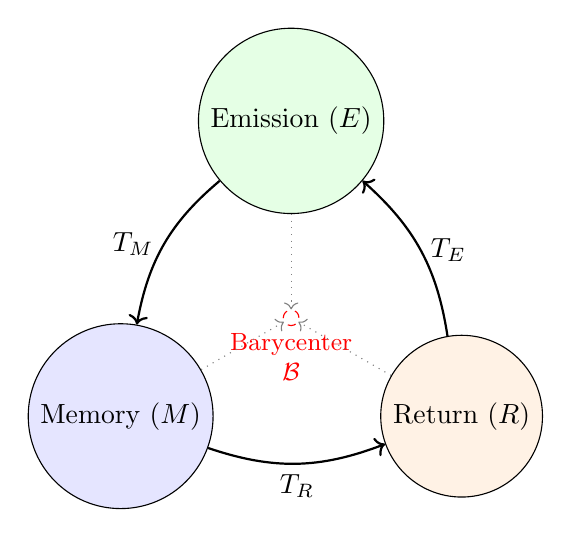
\begin{tikzpicture}
      % Triangle Nodes
      \node[draw, circle, fill=green!10] (E) at (90:2.5) {Emission ($E$)};
      \node[draw, circle, fill=blue!10] (M) at (210:2.5) {Memory ($M$)};
      \node[draw, circle, fill=orange!10] (R) at (330:2.5) {Return ($R$)};
      % Cycle Edges
      \draw[->, thick] (E) to[bend right=20] node[left] {$T_M$} (M);
      \draw[->, thick] (M) to[bend right=20] node[below] {$T_R$} (R);
      \draw[->, thick] (R) to[bend right=20] node[right] {$T_E$} (E);
      % Barycenter
      \node[draw=red, dashed, circle, inner sep=2pt] (B) at (0,0) {};
      \node[red, align=center, font=\small] at (0,-0.5) {Barycenter\\$\mathcal{B}$};
      % Convergence paths
      \draw[dotted, ->, gray] (E) -- (B);
      \draw[dotted, ->, gray] (M) -- (B);
      \draw[dotted, ->, gray] (R) -- (B);
    \end{tikzpicture}
    \caption{Triadic Convergence stabilizing into a 3-phase Barycentric Structure.}
    \label{fig:barycentric_structure}
\end{figure}

\begin{definition}[Triadic Convergence and Halting]
A triadic system is said to \textit{converge} if there exists a cycle index $k_0$ such that for all $k > k_0$:
\begin{enumerate}
    \item \textbf{Interval Minimization}: The width between the bounding mediants reaches the discrete floor:
    \[
    W(L_k, U_k) = \frac{1}{d_L d_U} \quad (\text{i.e., } \Delta_{\text{cross}} = 1).
    \]
    \item \textbf{Cycle Locking}: The state $s_k$ cycles strictly between the 3 distinct Barycentric Limits.
\end{enumerate}
\textbf{Halting Criterion}: The algorithm considers the value "computed" at step $k$ if the width condition $W=1$ is maintained for one full triadic period (3 steps).
\end{definition}

\section{The Translation Dictionary: Mapping Continuum Physics to Discrete Dynamics}

To utilize Rigbyspace Dynamics as a computational tool, one must translate continuum formulations into their constructive integer counterparts.

\subsection{Variable Translation}
\begin{table}[h!]
    \centering
    \renewcommand{\arraystretch}{1.5}
    \begin{tabular}{|p{4cm}|p{4cm}|p{6cm}|}
    \hline
    \textbf{Continuum Concept} & \textbf{Discrete Object} & \textbf{Rigbyspace Definition} \\
    \hline
    Continuous Time $t$ & Sequence $k \in \mathbb{Z}$ & Ordering index of evolution steps. \\
    \hline
    Coordinate $x$ & Rational Pair $s \in S_L$ & Explicit Rational Pair $(n, d)$. \\
    \hline
    Magnitude $|x|$ & Rank $\rho(x)$ & Structural depth via doubling thresholds. \\
    \hline
    Energy $E$ & Frequency $\Omega_{\text{vac}}$ & Count of vacuum generator iterations. \\
    \hline
    Phase $\theta$ & Discrete Phase $\phi$ & State in a finite cyclic graph $\Phi_N$. \\
    \hline
    \end{tabular}
    \caption{Dictionary of Fundamental Variables.}
\end{table}

\subsection{Structural Translation}
\subsubsection{Symmetry Groups vs. Phase Cycles}
Standard physics relies on Lie groups (e.g., $U(1)$). Rigbyspace replaces these with \textbf{Finite Phase Cycles}.
\begin{itemize}
    \item \textbf{Rotation}: Replaced by iterating the successor map on $\Phi_N$.
    \item \textbf{Gauge Invariance}: Replaced by Observational Equivalence ($\sim$) on $S_L$.
\end{itemize}

\subsubsection{Worked Translation Example: The Harmonic Oscillator}
\textbf{Problem}: Translate $\ddot{x} + \omega^2 x = 0$.
\textbf{Step 1}: Identify $x \to s_k \in S_L$. Restoring force $\to$ Phase Space map.
\textbf{Step 2}: The restoring force is modeled by the Transformative Reciprocal $\psi$ acting on the coupled pair $(x, p)$.
\textbf{Step 3}: The system evolves via the Triadic Map $s_{k+1} = T_{\phi(k)}(s_k)$, producing a Barycentric Oscillation.

\section{Coupled Systems: Matter-Vacuum Interaction}

\subsection{The Vertex State}
An interaction event is defined as a composite state where Matter and Vacuum share a boundary.
\[ \Psi_{\text{vertex}} := (P, L) \in S_P \times S_L \]

\subsection{Conservation of Rank}
In a closed interaction, total structural resources are conserved:
\[ \rho_{\text{total}}(\Psi) := \rho(P) + \rho(L). \]

\subsection{Interaction Cycle}
\begin{enumerate}
    \item \textbf{Matter Excitation}: $P' = P \boxplus P$. (Rank deficit created).
    \item \textbf{Tension Generation}: $T = \rho(P') - \rho(P)$.
    \item \textbf{Vacuum Resolution}: $L$ evolves via $G^{(k)}$ until $\Delta \rho \ge T$.
    \item \textbf{Vertex Update}: $\Psi_{\text{new}} = (P', L')$.
\end{enumerate}

\subsection{Scattering and Exchange}
A scattering event is defined as a swap of Vacuum components mediated by $\psi$:
\[ \text{Scattering}(\Psi_A, \Psi_B) := ((P_A, L_B), (P_B, L_A)) \]

\section{Lattice Topology and Cosmology}

\subsection{The Universal Graph}
The universe is defined as a directed graph $G$ where vertices are states and edges are valid transitions.
\[ U := (V, E) \]

\subsubsection{The Horizon}
The Computational Horizon is a complexity bound defined by the maximum rank $N$ the system can maintain without decoherence.
\[ H_{\text{max}} = \{ s \in S_L \mid \rho(s) \le N_{\text{crit}} \} \]

\subsection{Cosmological Expansion}
Cosmic expansion is the growth of the Phase Space modulus $N$.
\[ N(t+1) > N(t) \]
This allows for higher-rank states to exist, increasing the information capacity of the universe.

\subsubsection{Redshift Mechanism}
As $N$ increases, the relative density of low-rank states decreases. A signal emitted at modulus $N_{\text{old}}$ and received at $N_{\text{new}}$ appears redshifted due to the shifted rank structure.

\subsection{Boundary Conditions}
\begin{itemize}
    \item \textbf{Lower Bound}: The unit state $(1, 1)$. Provides a natural UV cutoff.
    \item \textbf{Upper Bound}: Defined by Vacuum Resolution Frequency latency. Regions where latency exceeds cycle time freeze (Event Horizon).
\end{itemize}

\subsection{Topological Defects}
Singularities manifest as graph defects:
\begin{itemize}
    \item \textbf{Monopoles}: Unbalanced inflow/outflow vertices.
    \item \textbf{Domain Walls}: Boundaries between Phase Space moduli.
    \item \textbf{Textures}: Twisted barycentric cycles.
\end{itemize}

\section*{Glossary of Terms}
\addcontentsline{toc}{section}{Glossary of Terms}

\begin{description}
    \item[Aggregate Transform ($\eta$)] A linear Vacuum Generator defined by $\eta(n, d) = (n+d, n)$. It corresponds to the continued fraction operation $[1; \dots]$ and increases the rank of the state linearly.

    \item[Barycentric Structure] The stable limit object of a Triadic system. It is not a single scalar value but a cyclic set of Explicit Rational States $\{L_E, L_M, L_R\}$ that define the "center of mass" of the oscillation.

    \item[Constraint Vacuum ($V_c$)] A state of the form $(n, 0)$ with $n \neq 0$. It represents a suspension where the metric basis (denominator) is lost, but the magnitude history (numerator) is preserved. It requires resolution via the Transformative Reciprocal.

    \item[Constructive Remainder] An integer-only algorithm (Alg 7.1) replacing the modulo operator. It computes the residue of division through repeated subtraction, strictly adhering to finitistic principles.

    \item[Explicit Rational Pair (ERP)] An ordered integer tuple $(n, d) \in \mathbb{Z} \times \mathbb{Z}_{\geq 0}$ representing a rational structure. ERPs are never reduced to lowest terms; the unreduced components encode the structural history (entropy) of the state.

    \item[Doubling Generator] A polynomial Matter interaction (Case B) acting on the Projective State Space $S_P$. It maps a state $P$ to a new state $P \boxplus P$ with significantly increased rank, driving the growth of Structural Entropy.

    \item[Explicit Rational State ($S_L$)] The set of all valid ERPs with non-zero denominator, $\{(n, d) \in \mathbb{Z}^2 \mid d \neq 0\}$. This is the primary domain for Vacuum evolution.

    \item[Lattice Coupling Constant ($\alpha_{\text{lat}}$)] The discrete analogue of the fine-structure constant. It is the asymptotic ratio of Transformative Reciprocal operations (interactions) to total vacuum propagation steps in a closed cycle.

    \item[Linear Transform ($\lambda$)] A linear Vacuum Generator defined by $\lambda(n, d) = (n+d, d)$. It increments the magnitude without altering the potential.

    \item[Mass-Gap Postulate] Axiom 10.1, stating that the universe consists of two distinct phases: Vacuum (linear/additive growth) and Matter (polynomial/multiplicative growth).

    \item[Null State] The state $(0,0)$. It contains no magnitude and no history. In ZERO Logic, it acts as an invariant sink that cannot be resolved into valid matter.

    \item[Numerical ZERO] A valid physical state of the form $(0, d)$ with $d > 0$. It has zero magnitude but possesses non-zero Structural Entropy $\rho(d)$.

    \item[Phase Space ($\Phi_N$)] The discrete replacement for the modulo operation. A finite set of integer states $\{0, \dots, N-1\}$ governed by a deterministic successor map.

    \item[Projective Curvature Constant ($K_{\text{proj}}$)] An integer triplet representing the minimal non-trivial deviation generated by a Matter interaction, providing a discrete measure of curvature.

    \item[Projective State Space ($S_P$)] The domain of Matter evolution, defined as integer triples $(X, Y, Z)$ where all components are non-zero. Evolution in $S_P$ is governed by polynomial maps.

    \item[Rank Function ($\rho$)] The discrete replacement for the logarithm. It measures the structural depth of an integer by counting the number of doubling thresholds $T_k = 2^k$ it has crossed.

   \item[Structural Entropy ($S$)] A measure of the causal history of a state, defined as the discrete rank of its geometric capacity (denominator): $S(s) = \rho(d)$. This measure quantifies the structural depth of the state's metric basis.

    \item[Successor-with-Reset] The fundamental operator on Phase Space $\Phi_N$ that increments the state and deterministically resets to 0 upon reaching $N-1$.

    \item[Suspended State] A state containing a Constraint Vacuum component. Evolution is paused (suspended) until a Transformative Reciprocal operator restores the metric basis.

    \item[Transformative Reciprocal ($\psi$)] The fundamental swap operator defined on coupled states: $\psi((a,b), (c,d)) = ((d,a), (b,c))$. It is the sole mechanism for resolving Constraint Vacuum singularities and generating reciprocal limits.

    \item[Triadic Convergence] The process by which a system settles into a stable 3-phase cycle (Emission, Memory, Return) rather than a single limit point.

    \item[Vacuum Resolution Frequency ($\Omega_{\text{vac}}$)] The integer count of vacuum generator applications required to balance a specific tension or curvature constraint. It replaces the continuum notion of energy.

    \item[Viscosity Sum] The accumulated phase drift of a system over a closed cycle. It represents the discrete manifestation of gravitational curvature.

    \item[ZERO Logic] The set of axioms and definitions governing the behavior of zero components, distinguishing between Numerical ZERO (valid magnitude), Constraint Vacuum (suspension), and Null State (collapse).
\end{description}

\end{document}

\subsection{Axioms for ZERO Logic}
\begin{axiom}[ZERO Determinism]
Operations applied to a Constraint ZERO do not produce undefined results. They produce a well-defined \emph{suspended state}.
\end{axiom}
\begin{axiom}[Numerator Conservation]
For any operation applied to a vacuum state, the numerator component is preserved. This ensures ZERO Logic is non-destructive.
\end{axiom}